\documentclass[12pt]{article}

\addtolength{\textwidth}{1.3in}
\addtolength{\oddsidemargin}{-.65in} %left margin
\addtolength{\evensidemargin}{-.65in}
\setlength{\textheight}{9in}
\setlength{\topmargin}{-.5in}
\setlength{\headheight}{0.0in}
\setlength{\footskip}{.375in}
\renewcommand{\baselinestretch}{1.0}
\renewcommand{\thesection}{\Roman{section}} 
\renewcommand{\thesubsection}{\thesection.\Roman{subsection}}
\linespread{1.5}

\usepackage[pdftex,
bookmarks=true,
bookmarksnumbered=false,
pdfview=fitH,
bookmarksopen=true]{hyperref}
\usepackage[pdftex]{graphicx}
%\usepackage{pdfpages}

\usepackage[usenames,dvipsnames,svgnames,table]{xcolor}
\usepackage{cite}
\usepackage{times, verbatim,bm,pifont,pdfsync}
%\usepackage[hang,flushmargin]{footmisc}%unindents footnotes

% disables chapter, section and subsection numbering
%\setcounter{secnumdepth}{-1} 

\usepackage{amsbsy,amssymb, amsmath, amsthm, MnSymbol,bbding}
\usepackage[hang,flushmargin]{footmisc} 

\newtheorem{definition}{Definition}
\newtheorem{theorem}{Theorem}
\newtheorem{lemma}{Lemma}
\newtheorem{corollary}{Corollary}
\newtheorem{assumption}{Assumption}
\newtheorem{fact}{Fact}
\newtheorem{result}{Result}
\newtheorem{proposition}{Proposition}

\newcommand{\ve}{\theta}
\newcommand{\ta}{\theta}
\newcommand{\ov}{\overline}
\newcommand{\un}{\underline}
\newcommand{\al}{\alpha}
\newcommand{\Ta}{\Theta}
\newcommand{\expect}{\mathbb{E}}
\newcommand{\Bt}{B(\bm{\tau^a})}
\newcommand{\bta}{\bm{\tau^a}}
\newcommand{\bte}{\bm{\tau^E}}
\newcommand{\btn}{\bm{\tau^n}}
\newcommand{\ga}{\gamma}


\begin{document}
\title{\vskip-0.6in LOBBYING AND LEGISLATIVE UNCERTAINTY}
\author{Kristy Buzard\thanks{Syracuse University, Economics Department, 110 Eggers Hall, Syracuse, NY 13244. Ph: 315-443-4079. Fax: 315-443-3717. Email: kbuzard@syr.edu. http://faculty.maxwell.syr.edu/kbuzard.} \and Sebastian Saiegh\thanks{University of California, San Diego, Department of Political Science, Social Sciences Building 365, 9500 Gilman Drive, La Jolla, CA 92093. Ph: 858-534-7237. Fax: 858-534-7130. Email: ssaiegh@ucsd.edu. http://pages.ucsd.edu/~ssaiegh/.}} 
\date{\vskip-.1in \today}
\maketitle

%\begin{center} {\bf Abstract} \end{center}

%\begin{quote}
%{\small This paper 

%\textit{JEL classification:} D72, D80 \\
%\textit{Keywords:} lobbying, political economy, legislatures, uncertainty}
%\end{quote}

\bigskip
\section{Introduction}
\label{sec:intro}

\textcolor{blue}{In democratic countries, legislatures are the authoritative source of statutory law. The PFS model doesn't capture several general features of policymaking in this environment: (2) how uncertainty affects the incentives for lobbying and the associated prospects for ratification of trade agreements; and (3) how the voting intentions of multiple legislators, rather than a single agent, change in response to incentives.}

\textcolor{blue}{In this vein, Saiegh (2011) identifies two major factors that shape lawmaking: the unpredictability of legislators' voting behavior, and whether buying legislative votes is a feasible option. The source of the uncertainty is the existence of cross-pressured legislators: in deciding how to vote, lawmakers consider a variety of influences, including their personal values, announced positions, the views of their constituents, and the preferences of their party leadership. Therefore, legislators' voting behavior can seldom be perfectly anticipated.}

\textcolor{blue}{From an empirical standpoint, the project will contribute to our understanding of the political uncertainty that surrounds statutory lawmaking. We will introduce an innovative methodology for quantifying cross-industry political uncertainty, establish the relevance of the resulting measures for policy-making and make the data available for future use in a wide range of applications. For example, our measure could be used to study he impact of policy uncertainty on firm-level investment and employment.}

\subsection{Related Literature}
\label{sec:lit}

\textcolor{blue}{Related is Le Breton and Salanie (2003), which studies lobbying when the lobby is uncertain about the preferences of a unitary decision maker. Le Breton and Zaporozhets (2007) go a step further and replace the unitary decision maker with a legislature with multiple actors. Song (2008) is a model of endogenous lobbying with a ratification constraint in a context of unilateral policy making with no uncertainty, and Coates and Ludema (2001) study trade policy leadership in a model with endogenous lobbying in the presence of political uncertainty with imperfect monitoring.}

\textcolor{blue}{As noted above, Saiegh (2009) argues that the uncertainty surrounding statutory lawmaking is in part related to governmental and political structure. Although they do not discuss uncertainty specifically, the cross-country empirical work of Gawande, Krishna and Olarreaga (2009) is the first to our knowledge that suggests that this kind of uncertainty plays a role in trade policy. They show that variables such as the number of checks and balances on the power of the legislature and the gap between the policy positions of the main political parties have predictive power for the PFS ``welfare-mindedness'' parameter. One of the objectives of this proposed project is to directly test the premise that legislative uncertainty indeed has an important impact on trade policy.}
			
\textcolor{blue}{This work also relates to the canonical studies on endogenous regulation (cf. Stigler (1975), Peltzman (1976), Becker (1983), Laffont and Tirole (1994)), as well as the literature on vote-buying and legislative behavior in political science (Groseclose and Snyder (1996), Dekel et. al. (2005), Dal Bo (2007)).}

%I will begin by ... Section~\ref{sec:main} then ... In Section~ \ref{sec:example}, ... Section~\ref{sec:dis} explores .... Several extensions of the model are explored in Section~\ref{sec:ext} and Section~\ref{sec:concl} concludes.


\section{The Model}
\label{sec:model}

The model is based on Banks' (2000) model of vote buying in a legislature, which is in turn a discrete version of Groseclose and Snyder's (1996) model with a continuum of legislators. The major difference here is the addition of uncertainty about the legislator's ideal points.

Each of three legislators faces a choice between the status quo, $x$ and a new policy proposal $s$. The utility function of legislator $i$ is given by $v(i) = u_i(x) - u_i(s)$, which is measured in money units. Note that legislators only have preferences about how they vote, not over which alternative wins.

There are two vote buyers labeled $A$ and $B$ who each prefers to maximize the expected value of his preferred policy net of the bribes he has to pay. $A$ prefers policy $x$ and has willingness to pay (WTP) $W_A$ for $x$ measured in money and values $s$ at zero. $B$ prefers $s$and has WTP $W_B$ for $s$. Each vote buyer would prefer to concede the issue rather than pay more than his WTP.

Vote Buyer $A$ moves first, providing a bribe offer function $a_i$. $a_i$ is perfectly observable to Vote Buyer $B$ when he moves second and offers bribe offer function $b_i$. Each legislator takes these bribe offers as given and then votes for the alternative that maximizes her payoff. I assume unbribed legislators who are indifferent vote for $s$.

\subsection{Legislature}
Let us look first at the legislature. Each legislator $i$ decides whether to vote for $x$ or $s$ given her preference $i$, $a_i$ and $b_i$. Although legislators are ordered on the interval according to their ideal points $i$, there is acknowledged uncertainty surrounding their preferences. We take this uncertainty to vary by legislator and also potentially by issue area when we extend the model to account for multi-dimensional voting and vote-buying.

In order to keep the model tractable when introduing this uncertainty, we take the ideal point function to be linear in $i$. That is, legislator $i$'s ideal point is taken to be $\alpha -\beta i$. We model uncertainty by taking legislator $i$ to vote for $x$ if 
			  \[
				  v(i) = \alpha -\beta i + \ve_i + a_i - b_i > 0
				\]
		
Notice that a bribe from $B$ is subtracted because it makes the alternative \textit{less} attractive.	We will begin by taking $\ve$ to not vary in $i$ and will shortly generalize.

Given these assumptions, the probability that legislator $i$ votes against the new proposal is
	\[
					\Pr\left[v(i)\leq 0 \right] = \Pr\left[\alpha -\beta i + \ve + a_i - b_i \leq 0 \right] = \Pr\left[\ve \leq \beta z - \alpha - a_i + b_i \right] 
	\]
Assuming $\ve \sim \text{Logistic} \ (0,1)$, the probability that legislator $z$ votes ``no'' is $\frac{1}{1+e^{-\left(\beta i - \alpha - a_i + b_i \right)}}$.	Whether a legislator $i$ votes ``no'' is a random variable, denote it $Q(i)$, distributed Bernoulli with this probability:
	\[
		Q(i) \sim \text{Bernoulli}(p(z)) \hskip.2in \text{where} \hskip.2in p(z) = \frac{1}{1+e^{-\left(\beta z - \alpha -a_i+ b_i \right)}}
	\]

For ease of exposition, for now take $i \in \left\{ -\frac{1}{2}, 0, \frac{1}{2} \right\}$. Then $Y_B = \frac{\beta}{2} - \alpha - a_{-\frac{1}{2}} + b_{-\frac{1}{2}}$, $X_B = -\alpha - a_0+ b_0$ and $Z_B = -\frac{\beta}{2} - \alpha - a_{\frac{1}{2}} + b_{\frac{1}{2}}\label{page:sh}$ represent the net ideal points in terms of $B$'s probability of winning the issue. We can then write the probability that each of the legislators, respectively, votes against the new proposal as $\frac{1}{1+e^{-Y_B}}$, $\frac{1}{1+e^{-X_B}}$ and $\frac{1}{1+e^{-Z_B}}$.

Vote Buyer $A$ must take into account that Vote Buyer $B$ will react to her choice of bribes. So the net ideal points from her point of view---that is, in terms of her winning the issue---are $X_A = \alpha - b_0(\bm{a},W_B,\al,\beta) + a_0$, $Y_A = -\frac{\beta}{2} + \alpha - b_{-.5}\left(\bm{a},W_B,\al,\beta\right)+ a_{-.5}$, and $Z_A = \frac{\beta}{2} + \alpha - b_{.5}\left(\bm{a},W_B,\al,\beta\right)+ a_{.5}$ with $\bm a = \left(a_{-.5},a_0,a_{.5} \right)$. We can then write the probability that each of the legislators votes for the new proposal as $\frac{1}{1+e^{-Y_A}}$, $\frac{1}{1+e^{-X_A}}$ and $\frac{1}{1+e^{-Z_A}}$.
				

\subsection{Vote Buyer B}
Groseclose and Snyder (1996) assume that the objective of each vote buyer is to ``minimize total bribes paid while passing his preferred policy.'' This has to be adapted out our environment with uncertainty about legislators' ideal points. The appropriate analog is that vote buyers maximize the expected value of winning the vote net of bribes that he/she must pay. Note that in order to maximize the probability of winning a majority in a three-seat legislature, one must maximize the probability of at least two legislators voting with you. The case of Vote Buyer $B$, this is the probability that at least two legislators vote in favor of the status quo: $\Pr(S \geq 2)$ where $S = X\left(-\frac{1}{2}\right) + X\left(0\right) + X\left(\frac{1}{2}\right)$.

This means that the maximization problem for Vote Buyer B (in absence of Vote Buyer A) is
			  \begin{multline}
			    \max_{b_{-\frac{1}{2}}, b_0, b_{\frac{1}{2}}} 
					W_B \biggl[ \Pr\left(X\left(-\frac{1}{2}\right)=1\right)\Pr\left(X\left(0\right)=1\right)\left(X\left(\frac{1}{2}\right)=0\right)  + \\
					\Pr\left(X\left(-\frac{1}{2}\right)=1\right)\Pr\left(X\left(0\right)=0\right)\Pr\left(X\left(\frac{1}{2}\right)=1\right) + \\
					\Pr\left(X\left(-\frac{1}{2}\right)=0\right)\Pr\left(X\left(0\right)=1\right)\Pr\left(X\left(\frac{1}{2}\right)=1\right) + \\
					\Pr\left(X\left(-\frac{1}{2}\right)=1\right)\Pr\left(X\left(0\right)=1\right)\Pr\left(X\left(\frac{1}{2}\right)=1\right) \biggr] - \sum_{j\in \left\{-\frac{1}{2}, 0,\frac{1}{2}\right\}} b_j
				\end{multline}
			Substituting from the definition of $X$,
			  \begin{multline}
			    \max_{b_{-\frac{1}{2}}, b_0, b_{\frac{1}{2}}} 
					W_B \biggl[ \frac{1}{1+e^{-Z}} \frac{1}{1+e^{-X}} \left(1-\frac{1}{1+e^{-Y}}\right)  + \\
					\frac{1}{1+e^{-Z}} \left(1-\frac{1}{1+e^{-X}}\right) \frac{1}{1+e^{-Y}} + \\
					\left(1-\frac{1}{1+e^{-Z}} \right) \frac{1}{1+e^{-X}} \frac{1}{1+e^{-Y}} + \\
					\frac{1}{1+e^{-Z}} \frac{1}{1+e^{-X}} \frac{1}{1+e^{-Y}} \biggr] - \sum_{j\in \left\{-\frac{1}{2}, 0,\frac{1}{2}\right\}} b_j
				\end{multline}
			This can be simplified as 
			  \begin{multline}
			    \max_{b_{-\frac{1}{2}}, b_0, b_{\frac{1}{2}}} 
					W_B \biggl[ \frac{1}{1+e^{-X}} \frac{1}{1+e^{-Y}} +
					\frac{1}{1+e^{-X}} \frac{1}{1+e^{-Z}} + \\
					\frac{1}{1+e^{-Y}} \frac{1}{1+e^{-Z}} - 2	\frac{1}{1+e^{-Z}} \frac{1}{1+e^{-X}} \frac{1}{1+e^{-Y}} \biggr] - \sum_{j\in \left\{-\frac{1}{2}, 0,\frac{1}{2}\right\}} b_j
					\label{eq:objb}
				\end{multline}
		
\subsection{Vote Buyer A}
Vote buyer A's objective function is identical in form to that of Vote buyer B (Expression~\ref{eq:objb}) 
			  \begin{multline}
			    \max_{a_{-\frac{1}{2}}, a_0, a_{\frac{1}{2}}} 
					W_A \biggl[ \frac{1}{1+e^{-X_A}} \frac{1}{1+e^{-Y_A}} +
					\frac{1}{1+e^{-X_A}} \frac{1}{1+e^{-Z_A}} + \\
					\frac{1}{1+e^{-Y_A}} \frac{1}{1+e^{-Z_A}} - 2	\frac{1}{1+e^{-Z_A}} \frac{1}{1+e^{-X_A}} \frac{1}{1+e^{-Y_A}} \biggr] - \sum_{j\in \left\{-\frac{1}{2}, 0,\frac{1}{2}\right\}} a_j .
					\label{eq:obja}
				\end{multline}

However, strategically Vote Buyer A is more complex because of the dependence of Vote Buyer $B$'s bids on her own.
				
\subsection{Non-negativity Constraints for Bribes}
\label{sec:nonneg}
It is not possible for a Vote Buyer to extract money from a legislator who is more favorably-inclined toward him than is optimal. This means that there are non-negativity constraints on all bribes. 

The Lagrangian for the problem is the same as Expression~\ref{eq:objb}, with the addition of three terms for the non-negativity constraints: $\lambda_X b_0 + \lambda_Y b_{-\frac{1}{2}} + \lambda_Z b_{\frac{1}{2}}$. Thus the full set of first order conditions are
\[
    W_B\frac{e^{-X}}{\left(1+e^{-X}\right)^2}\left[\frac{e^{-Z} + e^{-Y}}{\left(1+e^{-Z}\right)\left(1+e^{-Y}\right)} \right] - 1 + \lambda_X = 0
\]
\[
    W_B\frac{e^{-Y}}{\left(1+e^{-Y}\right)^2}\left[\frac{e^{-X} + e^{-Z}}{\left(1+e^{-X}\right)\left(1+e^{-Z}\right)} \right] - 1 + \lambda_Y = 0 
\]
\[
    W_B\frac{e^{-Z}}{\left(1+e^{-Z}\right)^2}\left[\frac{e^{-X} + e^{-Y}}{\left(1+e^{-X}\right)\left(1+e^{-Y}\right)} \right] - 1 + \lambda_Z = 0
\]
\[
  b\left(0\right) \geq0 \hskip.2in b\left(\frac{1}{2}\right) \geq0 \hskip.2in b\left(-\frac{1}{2}\right) \geq0 
\]
\[
  \lambda_X \geq0 \hskip.2in \lambda_Y \geq0 \hskip.2in \lambda_Z \geq0 
\]
\[
  \lambda_X \cdot b\left(0\right) = 0 \hskip.2in \lambda_Y \cdot b\left(-\frac{1}{2}\right) = 0 \hskip.2in \lambda_Z \cdot b\left(\frac{1}{2}\right) = 0 
\]



\subsection{Varying Uncertainty across Legislators}
\label{sec:uncert}
We allow the amount of uncertainty regarding each legislator's ideal point to vary across legislators by letting the scale parameter of the logistic distribution be different for each legislator. A larger scale parameter is associated with greater variance and thus more uncertainty as to the legislator's ideal point. The objective function for Vote Buyer $B$ becomes
 \begin{multline}
    \max_{b_{-\frac{1}{2}}, b_0, b_{\frac{1}{2}}} 
					W_B \biggl[ \frac{1}{1+e^{-\frac{X}{s_0}}} \frac{1}{1+e^{-\frac{Y}{s_{-.5}}}} +
					\frac{1}{1+e^{-\frac{X}{s_0}}} \frac{1}{1+e^{-\frac{Z}{s_{.5}}}} + \\
					\frac{1}{1+e^{-\frac{Y}{s_{-.5}}}} \frac{1}{1+e^{-\frac{Z}{s_{.5}}}} - 2	\frac{1}{1+e^{-\frac{Y}{s_{-.5}}}} \frac{1}{1+e^{-\frac{X}{s_0}}} \frac{1}{1+e^{-\frac{Z}{s_{.5}}}} \biggr] - \sum_{j\in \left\{-\frac{1}{2}, 0,\frac{1}{2}\right\}} b_j
	\end{multline}

We will see that allowing for this asymmetric uncertainty changes the predictions of the model in important ways. To lay the groundwork for the results to coming in Section~\ref{sec:resunc}, let's look at how the cumulative probabilities change for the most extreme legislators when the mean of their ideal point distribution is fixed but the scale parameter increases.

First, how does the probability that the legislator at $0.5$ (the one who is most unfriendly to $B$) votes with $B$ change when $s_{.5}$ goes from 1 to 2 in the absence of bribes? When $s_{.5}$ is 1, the probability is $\frac{1}{1+e^{-\frac{Z}{s_{.5}}}} = \frac{1}{1+e^{-\frac{-.5}{1}}} = \frac{1}{1+e^{.5}} = 0.3775$. When $s_{.5}$ is 2, the probability is $\frac{1}{1+e^{-\frac{Z}{s_{.5}}}} = \frac{1}{1+e^{-\frac{-.5}{2}}} = \frac{1}{1+e^{.25}} = 0.4378$. That is, the probability that the least friendly legislator votes with $B$ \textit{rises} when the uncertainty surrounding her ideal point increases.

Now, how does the probability that the legislator at $-0.5$ (the one who is most friendly to $B$) votes with $B$ change when $s_{-.5}$ goes from 1 to 2? When $s_{-.5}$ is 1, the probability is $\frac{1}{1+e^{-\frac{Y}{s_{-.5}}}} = \frac{1}{1+e^{-\frac{.5}{1}}} = \frac{1}{1+e^{-.5}} = 0.6225$. When $s_{-.5}$ is 2, the probability is $\frac{1}{1+e^{-\frac{Y}{s_{-.5}}}} = \frac{1}{1+e^{-\frac{.5}{2}}} = \frac{1}{1+e^{-.25}} = 0.5622$. Here, the probability that the most friendly legislator votes with $B$ \textit{falls} when the uncertainty surrounding her ideal point increases.



\section{Some Theoretical Results}
\label{sec:res}

Although uncertainty is present in the environment under consideration here, information about that uncertainty is symmetric. Therefore the appropriate equilibrium notion is subgame perfect Nash equilibrium.

I begin by examining the subgame that begins when Vote Buyer $B$ makes his offer. This not only serves to elucidate the basic logic of the model; it will also serve as a baseline from which to examine the incentives of Vote Buyer $A$. For now, assume that the uncertainty about ideal points is the same across legislators.

In a legislature with three voters, Vote Buyer $B$ can choose to bribe all three legislators, two, one or none of the legislators. It is most instructive to begin with the case where he bribes two of the legislators.

\begin{proposition}
  When Vote Buyer $B$ pays bribes to exactly two legislators, the bribes are such that the two bribed legislators' ideal points net of the bribes are equalized. Which two voters are bribed depends on the bias parameter $\al$.
	\label{prop:2NNB}
\end{proposition}

All proofs are in the Appendix.

\begin{itemize}
				\item With asymmetric $v(z)$ or WTP parameters, it would be easy to get equilibria where only $A$ or $B$ buys votes. But we also have lots of outcomes where both buy votes.
			\item They can easily both have positive probability of winning. But what do we need for this to be an equilibrium in this three stage game?
			\item Uncertainty buys us a lot: no longer this knife edge condition of $A$ pushing to the point that $B$ buys no votes
			\item Note the non-negativity constraint means you can't extract money from a legislator who is past the FOC point in order to reallocate to another legislator
			\item Some legislators who are past FOC point will not be lobbied		

\end{itemize}

\vskip.5in
Vote Buyer A's first order condition with respect to $a_0$ is more complicated because of the dependencies on $\bm a$ (should probably double check this, but it makes sense)
			 \begin{multline}
					 \frac{e^{-X} + e^{-Z}}{\left(1+e^{-X}\right)\left(1+e^{-Z}\right)} \frac{e^{-Y}}{\left[1+e^{-Y}\right]^2} \frac{\partial b_{-.5}}{\partial a_0} + \\ 
					\frac{e^{-X} + e^{-Y}}{\left(1+e^{-X}\right)\left(1+e^{-Y}\right)} \frac{e^{-Z}}{\left[1+e^{-Z}\right]^2}\frac{\partial b_{.5}}{\partial a_0} + \\
					\frac{2+e^{-Y} + e^{-Z}}{\left(1+e^{-Y}\right)\left(1+e^{-Z}\right)} \frac{e^{-X}}{\left[1+e^{-X}\right]^2}\left[1 - \frac{\partial b_0}{\partial a_0} \right] = \frac{1}{W_A}
					\label{eq:focA}
				\end{multline}

\subsection{Intuition}
\begin{itemize}

		\item If $\al > 0$, legislators on average are biased against B.
			\begin{itemize}
				\item If $\al < 0$, legislators on average are biased in favor of B.
				\item If $\al$ is negative enough, bribe only legislator furthest to the left (most against B)
			\end{itemize}
		\item If $X_B,Y_B,$ or $Z_B$ is positive, it means the probability of legislator $0,-\frac{1}{2},$ or $\frac{1}{2}$ voting for the status quo / against the new proposal / with interest group B is greater than $0.5$.
\end{itemize}


\vskip.1in
Pattern more or less is to get the guy who is WHAT?
\begin{itemize}
	\item From looking at overlaided graphs of the pdfs (pdf-graph.R), it appears that the legislator who is chosen first is the one who has the most probability mass just to the left of 0 (it's probability mass to the right of zero that counts for winning the vote).
		\begin{itemize}
			\item But this is not quite right: sometimes the non-negativity constraint binds on the PDF of that variables (as in the case of $\al=-0.3$ and $W_B = 8$.
		\end{itemize}
\end{itemize}
		
\vskip.1in
The only intuition I see for why the next legislator is added in is that it's when the additional expense is justified by the increase in winning probability, conditional on the rule that 2+ legislators have to have the same gross ideal point
\begin{itemize}
	\item I think it's actually that the next legislator is added when the non-negativity constraint stops binding; that is, when $W_B$ becomes high enough that the additional probability of winning is worth the additional cost
	\item What's the intuition for why they should be equal? As far as I can tell, it's that the PDF is unimodal. If the ideal points are very close, you don't want to continue moving one and leave the other behind because the marginal increase will be greater for whichever is to the left.
	\item \textbf{Next question: How general is this result? That is, how much asymmetry can I have in the logistic distribution, $\beta$s, and for how broad a class of distributions would it hold? My conjecture is that it leans on having an interior single mode}
\end{itemize}

\subsection{Varying Uncertainty across Legislators}
\label{sec:resunc}
Numerical example. Take $\al=0$ and ignore A. Take $s_{.5}$ from 1 to 1.5. $B$ stops bribing legislator $0.5$ (least friendly) altogether. Does better in welfare terms because the probability this guy votes in his favor shifts up
		\begin{itemize}
			\item For $s_{.5} = 1.1$, no bribe for $0.5$ guy until $W_B$ gets significantly higher, and then his net position is lower than $X=Y$
			\item At $s_{.5} = .75$: ONLY Z for $W_B \in \left[6,8\right]$ (8 is usually where it's $X$ alone). Then $Z$ and $Y$ together but $Z$ further on net than $Y$. Eventually all three, with $X=Y$, $Z$ further
		\end{itemize}
Numerical example. Take $\al=0$ and ignore A. Take $s_{-.5}$ from 1 to 2. $B$ stops bribing legislator $-0.5$ (most friendly) altogether.
		\begin{itemize}
			\item This is true even with $s_{-.5}$ as low as 1.2 (taking $s_{.5} = s_{0} = 1$)
			\item For $1 < s_{-.5} < 1.2$, no bribe for $-0.5$ guy until $W_B$ gets significantly higher, and then his net position is lower than $X=Z$
			\item Reverse if $s_{-.5} < 1$: move $-0.5$ guy further left than $X=Z$ (but not further than $X$ when just these two); in some cases leave $0.5$ guy at zero
		\end{itemize}
		
\section{Estimating Legislative Uncertainty}
\label{sec:est}

\textcolor{blue}{Recorded votes in legislatures (roll call data) are the most commonly used data source to measure politicians' spatial preferences. A well-established strategy is to use statistical techniques to represent patterns of legislative voting. The intuition behind these statistical models is that each roll call presents each legislator with a choice between a ``yea'' and a ``nay'' position. Legislators are presumed to vote for the position most similar to their own ideal policy position. As Clinton et al. (2004) note, it is possible to use Bayesian Markov chain simulation statistical methods to generate these preference estimates. This approach treats the unknown ideal points, bill parameters and legislators' utilities as random variables and condition upon the observed roll call data. The strategy is to impute values to these variables and estimate by regression the ideal points and bill parameters. The MCMC algorithm repeatedly performs these imputations and regressions and generates a large number of samples from the posterior density of the model parameters. Using this estimation procedure, we obtain summary statistics used for inference: legislators' mean and median ideal points as well as their 95$\%$ posterior confidence intervals. The latter are of particular interest to us, as we can use them to gauge the unpredictability of  legislators' voting behavior.}

\textcolor{blue}{We are interested in unpredictability vis-a-vis particular policy issues. Poole (2005) suggests using subsets of roll calls to establish legislators' ideal points separately on each issue. Preliminary work with our data indicates that a more statistically-robust method is to use all roll call votes in a legislative session or group of sessions to estimate an ideal point that is multidimension---that is, with one dimension for each interest group---allowing the partial pooling of information across roll calls. Multilevel modeling techniques, of which the standard ideal point estimation is a basic case, are perfectly suited to this task.}

\textcolor{blue}{We therefore estimate the model
\begin{equation}
  \Pr(y_{kj} = 1) = \text{logit}^{-1}\left( \sum_{g=1}^G \ga_k^{(g)}\left( \alpha_j^{(g)} - \beta_k^{(g)}\right) \right)
	\label{eq:v2}
\end{equation}
with roll call votes numbered $k=1,\ldots,K$, legislators numbered $j=1,\dots,J$, and interest groups numbered $g=1,\dots,G$. $y_{jk}=1$ if legislator $j$ votes ``Yea'' on bill $k$; $y_{kj}=0$ if she votes ``Nay'' on bill $k$. Note that interest groups take positions on multiple roll call votes and different interest groups can take positions, often on opposing sides, on each vote.}
		
\textcolor{blue}{This is a logistic item response (Rasch) model as adapted by Bafumi, et. al. (2005) to the legislative context. $\alpha_j^{(g)}$ is the ideal point of legislator $j$ on issue $g$ and $\beta_k^{(g)}$ is the ideal point of a legislator who is indifferent on vote $k$ for issue $g$. $\gamma_k^{(g)}$, the discrimination parameter, is a measure of the informativeness of issue $g$ for the vote on bill $k$: a large $\ga$ indicates that legislators are very likely to vote according to their preferences, whereas a small $\ga$ means that even significant margins of preference do not contribute much to the probability that legislators will vote in favor of the bill.}

\textcolor{blue}{We are experimenting with some of the more sophisticated measures of uncertainty that are possible with a rich model such as this one; for instance the group mean for $\ga$ and constructs that combine model parameters.}


\section{An Application to the U.S. House of Representatives}
\label{sec:house}

\subsection{Data}
\textcolor{blue}{Voting data will be obtained from Vote View, a website maintained by Professor Keith Poole (\url{http://voteview.com}). Details on each legislative proposal are available electronically through Thomas (\url{http://thomas.loc.gov}) and the sites of the House and Senate registrars.}

\textcolor{blue}{We will use Maplight's contributions data, which provides evidence on public declarations by special interest groups to determine the relevant PAC contributions for the bills under consideration. In a related effort to better connect special interest activity to the intent of that activity, we will use data made available pursuant to the U.S. Lobbying Disclosure Act of 1995 and the Honest Leadership and Open Government Act of 2007 via the U.S. Senate Office of Public Records and the Office of the Clerk of the U.S. House of Representatives. This data is particularly useful because lobbyists must declare the issue area on which they lobbied.}

\textcolor{blue}{We will also explore whether there is a way to leverage the data and methodology of Lake and Millimet (2014b) that combine the contributions and lobbying data to improve precision, although there is a concern about the coarseness of the data that must be overcome.}

\subsection{Evidence}

\begin{figure}
\centering
\begin{minipage}{.5\textwidth}
  \centering
  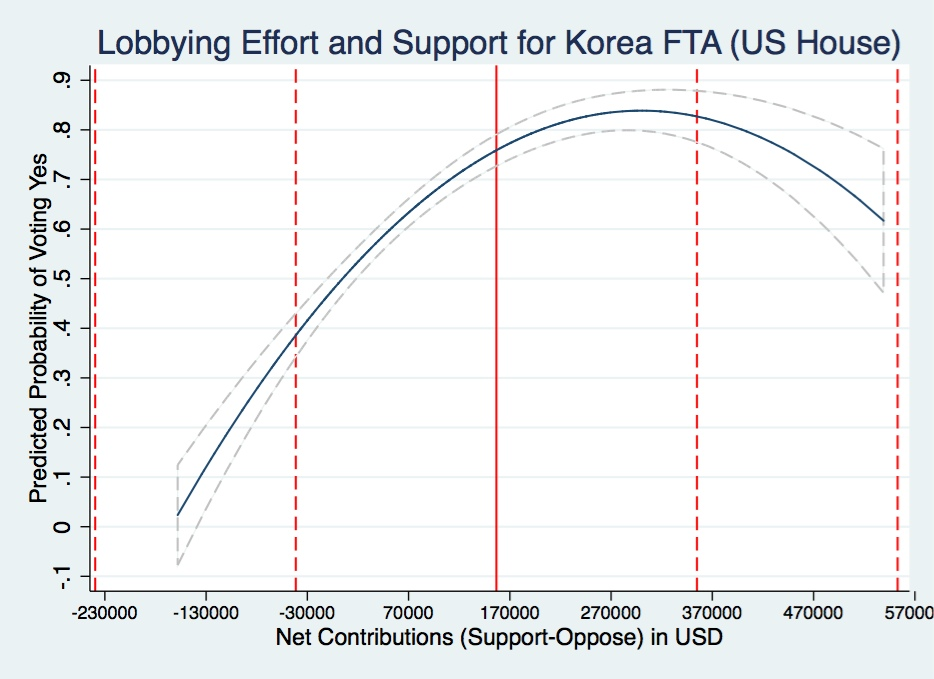
\includegraphics[width=2.9in]{graph2.jpg}
  \caption{Lobbying Effort and Support for KORUS
	\label{fig:br}}
\end{minipage}%
\begin{minipage}{.5\textwidth}
  \centering
  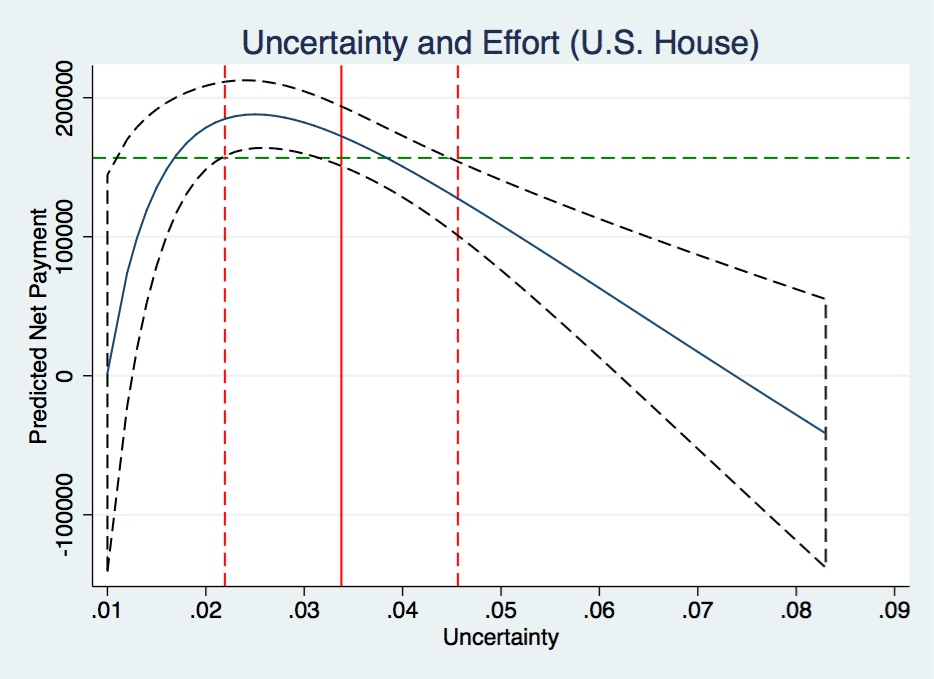
\includegraphics[width=2.9in]{graph1.jpg}
  \caption{Net Campaign Contributions, KORUS
	\label{fig:g1}}
\end{minipage}
\end{figure}

\textcolor{blue}{Figure~\ref{fig:br} displays the relationship between lobbying effort and legislators' support for KORUS. The vertical axis represents the predicted probability that a legislator would vote ``yes'' on the agreement, and the horizontal axis shows the monetary contributions to each legislator by lobbies who supported the passage of KORUS minus the contributions from lobbies opposing the agreement. The solid vertical red line indicates the average net contribution in the sample, and the dashed lines a one-standard deviation increase/decrease from that sample mean. The data indicate that exporting industries are more likely to exert lobbying effort to enlist the support of additional legislators (extensive margin) rather than secure stronger support from a given set of legislators (intensive margin), as well as that there are decreasing returns to lobbying effort. To generate these results,  we regressed a legislator's vote on his/her estimated ideal point as well as partisanship using a probit specification. Then we fitted a second-order polynomial to the predicted probabilities generated by the probit regression. The contribution data for both this and the follow figure was obtained from Maplight.}

\textcolor{blue}{Figure~\ref{fig:g1} displays the relationship between the unpredictability of legislators' voting behavior and lobbying effort. The vertical axis represents the predicted net contributions to members of the U.S. House of Representatives in 2012, and the horizontal axis shows the unpredictability of legislator's voting behavior measured using the 95$\%$ posterior confidence intervals of their ideal points estimated using Bayesian Markov chain simulation to scale all roll call votes taken in the 112th Congress (more details on the methodology below). The solid vertical red line indicates the average uncertainty in the sample, and the vertical dashed red lines indicate increases/decreases of one-standard deviation from the average. The horizontal dashed green line indicates the predicted net payment in the sample. The data show a very strong relationship between uncertainty at the level of the individual legislator and campaign contributions. To generate these results, we fitted a second-order polynomial to the data, and used monetary contributions to each legislator by lobbies who supported the passage of KORUS minus the contributions from lobbies opposing the agreement. While these data do not map perfectly onto our theoretical constructs, they indicate that there is strong preliminary support for our hypotheses making it highly likely that investment in data acquisition and analysis is worthwhile.}

\begin{figure}
\begin{center}
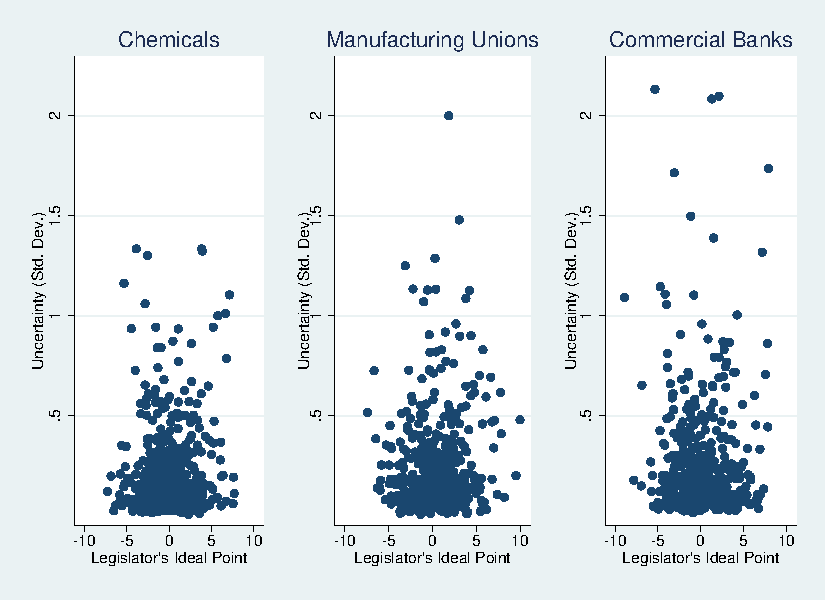
\includegraphics[height=3in, width=6.5in]{NSF_combined_graph.pdf}
\end{center}
\caption{Uncertainty by Industry\label{fig:combined}}
\end{figure}

\textcolor{blue}{We `turn on' the parameters for interest groups for each vote according to the data from Maplight, which includes a listing of the votes for which each interest group took a position. This produces estimates for how ``friendly'' or ``unfriendly'' each legislator is with respect to each interest group, as well as the unpredictability of his/her voting behavior when matters affecting that group are considered. In a preliminary run of this model with just ten interest groups (out of over 450) in the 112th Congress displayed in Figure~\ref{fig:combined}, we find that the chemical industry has the lowest average uncertainty (sd = 0.229); this is lower than the total uncertainty measure that can be interpreted as the standard left-right measure in ideal point models (sd = 0.233). The median group in terms of uncertainty is manufacturing unions (sd = 0.253), while construction equipment faced the highest uncertainty (sd = 0.285).}

\textcolor{blue}{Having created these measures of political uncertainty---which are entirely new to the best of our knowledge---we will proceed to characterize this uncertainty across industries, as well as how it is related to lobbying, political contributions and voting behavior of legislators. First, we want to understand the patterns in these data in the context of the industry-relevant bills identified by Maplight (as explained above).} 

\textcolor{blue}{We will use descriptive analysis as well as both standard parametric and non-parametric techniques such as density estimation to explore the relationships between the above variables of interest. We will begin with very basic questions such as whether distinct industries face varying levels of political uncertainty (see preliminary evidence in Figure~\ref{fig:combined}) and how those patterns may relate to the lobbying strategies they employ. From the data analysis that is represented above, we see a very interesting relationship between uncertainty and lobbying expenditure across legislators at the aggregate level in Figure~\ref{fig:br}, and we expect that additional important patterns will emerge when the data is disaggregated by industry.}



%\subsection{Break Decision}

%\subsection{Uncertainty for Select Interest Groups}
%\label{sec:select}


\section{Conclusion}
\label{sec:concl}

\textcolor{blue}{an alternative characterization of the legislative process would be one in which (i) bills have a quality dimension (such as their technical merit, or their appropriateness for a given situation); and (ii) legislators have access to different pieces of information about the quality of these proposals. Given our own long-term research agenda, adding common values and decentralized information to the analysis of the ratification of trade agreements will be one of the next steps in this project. Given the important set of governance characteristics identified in Mansfield and Milner (2012), we also look forward to taking advantage of what seems a rich opportunity to integrate important institutional variations into this modeling framework of endogenous lobbying with uncertainty.}

\vskip.3in
\textcolor{blue}{We expect this data will have a wide array of applications, such as exploring the links between policy uncertainty, the business cycle, and stock market volatility.}

\section*{Appendix}
\label{sec:app}
\noindent \textbf{\hypertarget{Pr_2NNB}{Proof of Proposition~\ref{prop:2NNB}}}: \\
Without loss of generality, assume that it is the legislators at $-\frac{1}{2}$ and $0$ that are bribed. The first order conditions with respect to the bribes for these two legislators are
	\begin{equation}
		\frac{e^{-X} + e^{-Z}}{\left(1+e^{-X}\right)\left(1+e^{-Z}\right)} \frac{e^{-Y}}{\left(1+e^{-Y}\right)^2}= \frac{1}{W_B}
	\end{equation}
	and
	\begin{equation}
		\frac{e^{-Y} + e^{-Z}}{\left(1+e^{-Y}\right)\left(1+e^{-Z}\right)} \frac{e^{-X}}{\left(1+e^{-X}\right)^2}= \frac{1}{W_B}
		\label{eq:base}
	\end{equation}
		
		Setting the left-hand size of these two equations equal to each other and simplifying,
		\[
		  \frac{e^{-Y} + e^{-Z}}{\left(1+e^{-Y}\right)\left(1+e^{-Z}\right)} \frac{e^{-X}}{\left(1+e^{-X}\right)^2}= \frac{e^{-X} + e^{-Z}}{\left(1+e^{-X}\right)\left(1+e^{-Z}\right)} \frac{e^{-Y}}{\left(1+e^{-Y}\right)^2}
		\]
		\[
		  \frac{e^{-X-Y} + e^{-X-Z}}{1+e^{-X}}= \frac{e^{-X-Y} + e^{-Y-Z}}{1+e^{-Y}}
		\]
		\[
		  e^{-X-Y} + e^{-X-Z} + e^{-X-2Y} +e^{-X-Y-Z}= e^{-X-Y} + e^{-Y-Z} + e^{-2X-Y} +e^{-X-Y-Z}
		\]
		\[
		  e^{-X-Z} +e^{-X-2Y}= e^{-Y-Z} +e^{-2X-Y}
		\]
		\[
		  e^{-Z} +e^{-2Y}= e^{X-Y-Z} +e^{-X-Y}
		\]
		\begin{equation}
		  e^{Y-Z} +e^{-Y}= e^{X-Z} +e^{-X}
			\label{eq:twoways}
		\end{equation}
   Equation~\ref{eq:twoways} can be rearranged into two similar forms. First:
		\[
		  e^{Y-Z} - e^{X-Z}= e^{-X} - e^{-Y}
		\]
		\begin{equation}
		  e^{Y} - e^{X}= e^Z\left(e^{-X} - e^{-Y}\right)
			\label{eq:1}
		\end{equation}
  	Second, multiplying through by zero:
	  \begin{equation}
		  e^{X} - e^{Y}= e^Z\left(e^{-Y} - e^{-X}\right)
			\label{eq:2}
		\end{equation}
		
In this case where the non-negativity constraint binds for the variable associated with $Z$, that is $b\left(-\frac{1}{2}\right)$, we know that $Z < 0$. Note that this is due to the construction of the problem. This means $e^Z < 1$. In this case,
	\begin{itemize}
		\item Equation~\ref{eq:1} is consistent with $X>Y>0$, $X>0>Y$, or $0>X>Y$.
		\item Equation~\ref{eq:2} is consistent with $Y>X>0$, $Y>0>X$, or $0>Y>X$.
	\end{itemize}
The second order conditions imply that both $X$ and $Y$ are positive, thus it must be that $X = Y > 0$. Note that once this is known, one can go back to, for instance, Equations~\ref{eq:base} and substitute for one of the variables. Given that $Z=0$, with a particular value of $\left(\alpha,W_B\right)$, the solution gives the values of the two relevant bribes.



\newpage
\section*{References}

\begin{list}{}{\setlength{\leftmargin}{0.3in}\setlength{\rightmargin}{0.0in}\setlength{\itemindent}{-0.3in}\setlength{\itemsep}{0.0in}}


\item Ansolabehere, S., J. de Figueiredo, and J. Snyder Jr. (2003), ``Why Is There so Little Money in U.S. Politics?,'' {\em Journal of Economic Perspectives}, 17, 105-130.

\item Banks, J. S., (2000), ``Buying Supermajorities in Finite Legislatures.'' {\em The American Political Science Review} 94, 677-681.

\item Becker, G., (1983), ``A Theory of Competition among Interest Groups for Political Influence.'' {\em Quarterly Journal of Economics} 98, 371-400.

\item Bombardini, M. (2008), ``Firm Heterogeneity and Lobby Participation,'' {\em Journal of International Economics}, 75, 329-348.

\item Bombardini, M., and F. Trebbi (2012): ``Competition and Political Organization: Together or Alone in Lobbying for Trade Policy?'' {\em Journal of International Economics}, 87, 18-26.

\item Clinton, J., Jackman, S., and D. Rivers, (2004): ``The Statistical Analysis of Roll Call Data.'' {\em American Political Science Review}, 98, 355-370.

\item Dal Bo, E. (2007): ``Bribing Voters.'' {\em American Journal of Political Science} 51, 789-803.

\item Dekel, E., Jackson, M., Wolinsky, A. (2005): {\em Vote Buying.} Unpublished manuscript, Caltech.

\item Gawande, K., P. Krishna and M. Robbins (2006): ``Foreign Lobbies and U.S. Trade Policy,'' {\em Review of Economics and Statistics}, 88, 563-571.

\item Goldberg, P. and G. Maggi (1999): ``Protection for Sale: An Empirical Investigation,'' {\em American Economic Review}, 89, 1135-1155.

\item Groseclose, T., Snyder, J. M. (1996): ``Buying Supermajorities.'' {\em American Political Science Review} 90, 303-315.

\item Grossman, G. and E. Helpman (1994): ``Protection for Sale,'' {\em The American Economic Review}, 84, 833-850.

\item Grossman, G. and E. Helpman (2005): ``A Protectionist Bias in Majoritarian Politics,'' {\em The Quarterly Journal of Economics}, 120, 1239-1282.

\item Henisz, W. and E. Mansfield (2006), ``Votes and Vetoes: The Political Determinants of Commercial Openness,'' {\em International Studies Quarterly}, 50, 189-211.

\item Kibris, A. (2012), ``Uncertainty and Ratification Failure,'' {\em Public Choice}, 150, 439-467.

\item Laffont, J., Tirole, J. (1994): ``A Theory of Incentives in Procurement and Regulation.'' Cambridge: MIT Press.

\item Laver, M. and K. Shepsle (1991), ``Divided Government: America is Not `Exceptional','' {\em Governance: An International Journal of Policy and Administration}, 4, 250-269.

\item Le Breton, M. and F. Salanie (2003), ``Lobbying under political uncertainty,'' {\em Journal of Public Economics}, 87, 2589-2610.

\item Le Breton, M. and V. Zaporozhets (2007), ``Legislative Lobbying under Political Uncertainty,'' Available at SSRN: \url{http://ssrn.com/abstract=1024686}.

\item Peltzman, S. (1976), ``Toward a More General Theory of Regulation.'' {\em Journal of Law and Economics} 19, 211-248.

\item Poole, K. T. (2005), ``Spatial Models of Parliamentary Voting.'' New York: Cambridge University Press.

\item Saiegh, S. (2009), ``Political  Prowess or Lady Luck? Evaluating Chief Executives' Legislative Success Rates,'' {\em The Journal of Politics}, 71, 1342-1356.

\item Saiegh, S. (2011) ``Ruling by Statute: How Uncertainty and Vote-Buying Shape Lawmaking.'' New York: Cambridge University Press.

\item Stigler, G. (1975) ``The Citizen and the State: Essays on Regulation.'' Chicago: Chicago University Press.



\item Bafumi, J., Gelman, A., Park., D, Kaplan, N., 2005. Practical Issues in Implementing and Understanding Bayesian Ideal Point Estimation. Political Analysis 13, 171-187.
	
	

	\item Buzard, K., 2014a. Endogenous Politics and the Design of Trade Agreements. Available at: \url{https://kbuzard.expressions.syr.edu/wp-content/uploads/Endogenous-Politics.pdf}.	
		
	\item Buzard, K., 2014b. Self-enforcing Trade Agreements, Dispute Settlement and Separation of Powers. Available at: \url{https://kbuzard.expressions.syr.edu/wp-content/uploads/2014/04/Self-enforcing-Trade_Agreements.pdf}.

\begin{sloppypar}	
	\item Buzard, K., 2014c. Trade Agreements in the Shadow of Lobbying. Available at: \url{https://kbuzard.expressions.syr.edu/wp-content/uploads/TradeAgreements_Shadow_Lobbying.pdf}.
		\end{sloppypar}
		

	\item Coates, D., Ludema, R., 2001. A Theory of Trade Policy Leadership. Journal of Development Economics 65, 1-29.
	
	\item Conconi, P., Facchini, G., Steinhardt, M. F., Zanardi, M., 2012. The political economy of trade and migration: Evidence from the US Congress. HWWI Research Paper 136. Available at: \url{http://hdl.handle.net/10419/67944}.
	
	\item Dixit, A., Grossman, G., Helpman, E., 1997. Common Agency and Coordination: General Theory and Application to Government Policy Making. Journal of Political Economy 105, 752-769.

	\item Feenstra, R., 1992. How Costly is Protectionism? Journal of Economic Perspectives 6, 159-178.

	\item Gawande, K., Bandyopadhyay, U., 2000. Is Protection for Sale? Evidence on the Grossman-Helpman Theory of Endogenous Protection. The Review of Economics and Statistics 82, 139-152.

	\item Gawande, K., Krishna, P., Olarreaga, M., 2009. What Governments Maximize and Why: The View from Trade. International Organization 63, 491-532.

	\item Gawande, K., Krishna, P., Olarreaga, M., 2012. Lobbying Competition over Trade Policy. International Economic Review 53, 115-132.

	\item Grossman, G., Helpman, E., 1995a. The Politics of Free-Trade Agreements. The American Economic Review 85, 667-690.

	\item Grossman, G., Helpman, E., 1995b. Trade Wars and Trade Talks. The Journal of Political Economy 103, 675-708.

	\item Iaryczower, M., Katz, G., Saiegh, S., 2013. Voting in the Bicameral Congress: Large Majorities as a Signal of Quality. Forthcoming in Journal of Law, Economics, and Organization.

  \item Iida, K., 1996. Involuntary Defection in Two-Level Games. Public Choice 89, 283-303.
  
	\item Lake, J., Millimet, D., 2014a. An Empirical Analysis of Trade-Related Redistribution and the Political Viability of Free Trade. Available at: \url{http://people.smu.edu/jlake/pdfs/VotingFTAs.pdf}

	\item Lake, J., Millimet, D., 2014b. Revisiting the link between PAC Contributions and Lobbying Expenditures. Available at: \url{http://people.smu.edu/jlake/pdfs/PACcontributionsLobbying.pdf}

	\item Mansfield, E., Milner, H., 2012. Votes, Vetoes, and the Political Economy of International Trade Agreements. Princeton and Oxford: Princeton  University Press.

	\item Milner, H., Rosendorff, B.P., 1997. Democratic Politics and International trade Negotiations: Elections and Divided Government as Constraints on Trade Liberalization. Journal of Conflict Resolution 41, 117-147.

	\item Ornelas, E., 2005. Rent Destruction and the Political Viability of Free Trade Agreements. Quarterly Journal of Economics 120, 1475-1506.

  

\end{list}

\end{document}